%!TEX root = ../dokumentation.tex

\RequirePackage[l2tabu, orthodox]{nag}	% weist in Commandozeile bzw. log auf veraltete LaTeX Syntax hin

\documentclass[%
    pdftex,
    oneside,			% Einseitiger Druck.
    12pt,				% Schriftgroesse
    parskip=half,		% Halbe Zeile Abstand zwischen Absätzen.
    %topmargin = 10pt,	% Abstand Seitenrand (Std:1in) zu Kopfzeile [laut log: unused]
    headheight = 33pt,	% Höhe der Kopfzeile
    %headsep = 30pt,	% Abstand zwischen Kopfzeile und Text Body  [laut log: unused]
    headsepline,		% Linie nach Kopfzeile.
    footsepline,		% Linie vor Fusszeile.
    %footheight = 16pt,	% Höhe der Fusszeile
    abstracton,		% Abstract Überschriften
    DIV=calc,		% Satzspiegel berechnen
    BCOR=8mm,		% Bindekorrektur links: 8mm
    headinclude=false,	% Kopfzeile nicht in den Satzspiegel einbeziehen
    footinclude=false,	% Fußzeile nicht in den Satzspiegel einbeziehen
    listof=totoc,		% Abbildungs-/ Tabellenverzeichnis im Inhaltsverzeichnis darstellen
    toc=bibliography,	% Literaturverzeichnis im Inhaltsverzeichnis darstellen
]{scrreprt}	% Koma-Script report-Klasse, fuer laengere Bachelorarbeiten alternativ auch: scrbook

% Einstellungen laden
\usepackage{xstring}

\usepackage{lastpage}
\usepackage{fancyhdr}
\newcommand{\einstellung}[1]{%
    \expandafter\newcommand\csname #1\endcsname{}
    \expandafter\newcommand\csname setze#1\endcsname[1]{\expandafter\renewcommand\csname#1\endcsname{##1}}
}
\newcommand{\langstr}[1]{\einstellung{lang#1}}

% Flag für die Selbstständigkeitserklärung, Default: true
\newif\ifselbsterkl
\selbsterklfalse

% Flag für das Wasserzeichen auf dem Deckblatt, default: false
\newif\ifwatermark
\watermarkfalse

% Flag für roten Vertraulichkeitspunkt, default: false
\newif\ifreddot
\reddotfalse

% Flag für gelben Vertraulichkeitspunkt, default: false
\newif\ifyellowdot
\yellowdotfalse

% Flag für das Unterschriftenblatt, default: false
\newif\ifunterschriftenblatt
\unterschriftenblattfalse

% Flag für Einfügen der Seitenzahl bei Verweis auf Kapitel/Abschnitt, default: false
\newif\ifrefWithPages
\refWithPagesfalse

% Flag für Einfügen der Abstracts in deutsch und englisch, default: false
\newif\ifbothabstracts
\bothabstractsfalse

% Flag für Einfügen des Abkürzungsverzeichnis
\newif\ifabkverz
\abkverzfalse

% Flag für Einfügen des Abbildungsverzeichnisses
\newif\ifabbverz
\abbverzfalse

% Flag für Einfügen des Formelverzeichnisses
\newif\ifformelverz
\formelverzfalse

% Flag für Einfügen des Formelgroessenverzeichnisses
\newif\ifformelgroeverz
\formelgroeverzfalse 

% Flag für Einfügen des Listingsverzeichnisses
\newif\iflistverz
\listverzfalse

% Flag für Einfügen des Tabellenverzeichnisses
\newif\iftableverz
\tableverzfalse

% Flag für Einfügen des Sperrvermerks
\newif\ifsperrvermerk
\sperrvermerkfalse

% Flag für Einfügen des Abstracts
\newif\ifabstract
\abstractfalse

% Flag für Anhang
\newif\ifappendix
\appendixfalse

% Flag für Literaturverzeichnis
\newif\ifliteratur
\literaturfalse

% Flag für Glossar
\newif\ifglossar
\glossarfalse

% Flag für Inhaltsverzeichnis
\newif\ifinhalt
\inhaltfalse

\einstellung{martrikelnr}
\einstellung{titel}
\einstellung{kurs}
\einstellung{datumAbgabe}
\einstellung{firma}
\einstellung{firmenort}
\einstellung{abgabeort}
\einstellung{abschluss}
\einstellung{studiengang}
\einstellung{dhbw}
\einstellung{betreuer}
\einstellung{gutachter}
\einstellung{zeitraum}
\einstellung{arbeit}
\einstellung{autor}
\einstellung{sprache}
\einstellung{schriftart}
\einstellung{kapitelabstand}
\einstellung{spaltenabstand}
\einstellung{zeilenabstand}
\einstellung{zitierstil}
\einstellung{selbsterkl}
 % verfügbare Einstellungen
%%%%%%%%%%%%%%%%%%%%%%%%%%%%%%%%%%%%%%%%%%%%%%%%%%%%%%%%%%%%%%%%%%%%%%%%%%%%%%%
%                                   Einstellungen
%
% Hier k�nnen alle relevanten Einstellungen f�r diese Arbeit gesetzt werden.
% Dazu geh�ren Angaben u.a. �ber den Autor sowie Formatierungen.
%
%
%%%%%%%%%%%%%%%%%%%%%%%%%%%%%%%%%%%%%%%%%%%%%%%%%%%%%%%%%%%%%%%%%%%%%%%%%%%%%%%


%%%%%%%%%%%%%%%%%%%%%%%%%%%%%%%%%%%% Sprache %%%%%%%%%%%%%%%%%%%%%%%%%%%%%%%%%%%
%% Aktuell sind Deutsch und Englisch unterst�tzt.
%% Es werden nicht nur alle vom Dokument erzeugten Texte in
%% der entsprechenden Sprache angezeigt, sondern auch weitere
%% Aspekte angepasst, wie z.B. die Anf�hrungszeichen und
%% Datumsformate.
\setzesprache{de} % oder en
%%%%%%%%%%%%%%%%%%%%%%%%%%%%%%%%%%%%%%%%%%%%%%%%%%%%%%%%%%%%%%%%%%%%%%%%%%%%%%%%

%%%%%%%%%%%%%%%%%%%%%%%%%%%%%%%%%%% Angaben  %%%%%%%%%%%%%%%%%%%%%%%%%%%%%%%%%%%
%% Die meisten der folgenden Daten werden auf dem
%% Deckblatt angezeigt, einige auch im weiteren Verlauf
%% des Dokuments.
\setzemartrikelnr{3394182, 7008632}
\setzekurs{STG-TINF17ITA}
\setzetitel{Verwendung von Eye-Tracking zur Steuerung von Bedienelementen in Virtual Reality}
\setzedatumAbgabe{-todo-}
\setzefirma{Robert Bosch GmbH}
\setzefirmenort{-todo-}
\setzeabgabeort{Stuttgart}
%\setzeabschluss{Bachelor of Engineering}
\setzestudiengang{-todo-}
\setzedhbw{Stuttgart}
\setzebetreuer{-todo-}
\setzezeitraum{Oktober 2019 - Juni 2020}
\setzearbeit{Studienarbeit}
\setzeautor{Clemens Mollik, J�rn Herbstritt}

\inhalttrue                 % auskommentieren oder �ndern zu \inhaltfalse, falls kein Inhaltsverzeichnis eingef�gt werden soll
\unterschriftenblattfalse    % auskommentieren oder �ndern zu \unterschriftenblattfalse, falls kein Unterschriftenblatt eingef�gt werden soll
\selbsterklfalse             % auskommentieren oder �ndern zu \selbsterklfalse, wenn keine Selbstst�ndigkeitserkl�rung ben�tigt wird
\sperrvermerkfalse           % auskommentieren oder �ndern zu \sperrvermerkfalse, wenn kein Sperrvermerk ben�tigt wird
\abkverztrue                % auskommentieren oder �ndern zu \abkverzfalse, wenn kein Abk�rzungsverzeichnis ben�tigt wird
\abbverztrue                % auskommentieren oder �ndern zu \abbverzfalse, wenn kein Abbildungsverzeichnis ben�tigt wird
\tableverztrue              % auskommentieren oder �ndern zu \tableverzfalse, wenn kein Tabellenverzeichnis ben�tigt wird
\listverztrue               % auskommentieren oder �ndern zu \listverzfalse, wenn kein Listingsverzeichnis ben�tigt wird
\formelverztrue             % auskommentieren oder �ndern zu \formelverzfalse, wenn kein Formelverzeichnis ben�tigt wird
\formelgroeverztrue			% auskommentieren oder �ndern zu \formelgroeverzfalse, wenn kein Formelgr��enverzeichnis ben�tigt wird
\abstracttrue               % auskommentieren oder �ndern zu \abstractfalse, wenn kein Abstract gew�nscht ist
\bothabstractstrue          % auskommentieren oder �ndern zu \bothabstractsfalse, wenn nur der Abstract in der Hauptsprache eingef�gt werden soll
\appendixtrue               % auskommentieren oder �ndern zu \appendixfalse, wenn kein Anhang gew�nscht ist
\literaturtrue              % auskommentieren oder �ndern zu \literaturfalse, wenn kein Literaturverzeichnis gew�nscht ist (\appendixtrue muss gesetzt sein!)
\glossartrue                % auskommentieren oder �ndern zu \glossarfalse, wenn kein Glossar gew�nscht ist (\appendixtrue muss gesetzt sein!)
\watermarkfalse             % auskommentieren oder �ndern zu \watermarktrue, wenn Wasserzeichen auf dem Titelblatt eingef�gt werden soll

\refWithPagesfalse          % �ndern zu \refWithPagestrue, wenn die Seitenzahl bei Verweisen auf Kapitel engef�gt werden sollen


% Angabe des roten/gelben Punktes auf dem Titelblatt zur Kennzeichnung der Vertraulichkeitsstufe.
% M�gliche Angaben sind \yellowdottrue und \reddottrue. Werden beide angegeben, wird der rote Punkt gezeichnet.
% Wird keines der Kommandos angegeben, wird kein Punkt gezeichnet
%\yellowdottrue

%%%%%%%%%%%%%%%%%%%%%%%%%%%%%%%%%%%%%%%%%%%%%%%%%%%%%%%%%%%%%%%%%%%%%%%%%%%%%%%%

%%%%%%%%%%%%%%%%%%%%%%%%%%%% Literaturverzeichnis %%%%%%%%%%%%%%%%%%%%%%%%%%%%%%
%% Bei Fehlern w�hrend der Verarbeitung bitte in ads/header.tex bei der
%% Einbindung des Pakets biblatex (ungef�hr ab Zeile 110,
%% einmal f�r jede Sprache), biber in bibtex �ndern.
\newcommand{\ladeliteratur}{%
\addbibresource{bibliographie.bib}
%\addbibresource{weitereDatei.bib}
}

%% Zitierstil
%% siehe: http://ctan.mirrorcatalogs.com/macros/latex/contrib/biblatex/doc/biblatex.pdf (3.3.1 Citation Styles)
%% m�gliche Werte z.B numeric-comp, alphabetic, authoryear
\setzezitierstil{alphabetic}
%%%%%%%%%%%%%%%%%%%%%%%%%%%%%%%%%%%%%%%%%%%%%%%%%%%%%%%%%%%%%%%%%%%%%%%%%%%%%%%%

%%%%%%%%%%%%%%%%%%%%%%%%%%%%%%%%% Layout %%%%%%%%%%%%%%%%%%%%%%%%%%%%%%%%%%%%%%%
%% Verschiedene Schriftarten
% laut nag Warnung: palatino obsolete, use mathpazo, helvet (option scaled=.95), courier instead
\setzeschriftart{lmodern} % palatino oder goudysans, lmodern, libertine

%% Abstand vor Kapitel�berschriften zum oberen Seitenrand
\setzekapitelabstand{20pt}

%% Spaltenabstand
\setzespaltenabstand{10pt}
%%Zeilenabstand innerhalb einer Tabelle
\setzezeilenabstand{1.5}
%%%%%%%%%%%%%%%%%%%%%%%%%%%%%%%%%%%%%%%%%%%%%%%%%%%%%%%%%%%%%%%%%%%%%%%%%%%%%%%% % lese Einstellungen

\newcommand{\iflang}[2]{%
  \IfStrEq{\sprache}{#1}{#2}{}
}

\langstr{abkverz}
\langstr{anhang}
\langstr{glossar}
\langstr{deckblattabschlusshinleitung}
\langstr{artikelstudiengang}
\langstr{studiengang}
\langstr{anderdh}
\langstr{von}
\langstr{dbbearbeitungszeit}
\langstr{dbmatriknr}
\langstr{dbkurs}
\langstr{dbfirma}
\langstr{dbbetreuer}
\langstr{dbgutachter}
\langstr{sperrvermerk}
\langstr{erklaerung}
\langstr{abstract}
\langstr{listingname}
\langstr{listlistingname}
\langstr{listingautorefname}
\langstr{selbsterkl}
\langstr{formelsammlung}
\langstr{kopfz}
\langstr{fussz}
\langstr{seite}
\langstr{seitevon}
\langstr{stand}
\langstr{formelgroeverz} % verfügbare Strings
\input{lang/\sprache} % Übersetzung einlesen


%\lstset{language=Matlab}
\newcommand{\citem}[1]{\item[\texttt{#1}]} % Code-Item für description-Liste
%\newcommand\todo[1]{\textit{\textcolor{red}{TODO: #1}}\message{LaTeX Warning: \noexpand TODO item left in line \the\inputlineno}} % Todo-Item
\newcommand\todo[1]{\textit{\textcolor{red}{TODO: #1}}} % Todo-Item
\usepackage{pdfpages}         % pdf-Seiten einbinden

%% Farben (Angabe in HTML-Notation mit großen Buchstaben)
\newcommand{\ladefarben}{%
	\definecolor{LinkColor}{HTML}{00007A}
	\definecolor{ListingBackground}{HTML}{FCF7DE}
}
%% Mathematikpakete benutzen (Pakete aktivieren)
%\usepackage{amsmath}
%\usepackage{amssymb}

%% Programmiersprachen Highlighting (Listings)
\newcommand{\listingsettings}{%
	\lstset{%
		language=C++,			% Standardsprache des Quellcodes
		%numbers=left,			% Zeilennummern links
		%stepnumber=1,			% Jede Zeile nummerieren.
		%numbersep=5pt,			% 5pt Abstand zum Quellcode
		%numberstyle=\tiny,		% Zeichengrösse 'tiny' für die Nummern.
		breaklines=true,		% Zeilen umbrechen wenn notwendig.
		breakautoindent=true,	% Nach dem Zeilenumbruch Zeile einrücken.
		postbreak=\space,		% Bei Leerzeichen umbrechen.
		tabsize=2,				% Tabulatorgrösse 2
		basicstyle=\ttfamily\footnotesize, % Nichtproportionale Schrift, klein für den Quellcode
		showspaces=false,		% Leerzeichen nicht anzeigen.
		showstringspaces=false,	% Leerzeichen auch in Strings ('') nicht anzeigen.
		extendedchars=true,		% Alle Zeichen vom Latin1 Zeichensatz anzeigen.
		captionpos=b,			% sets the caption-position to bottom
		%backgroundcolor=\color{ListingBackground}, % Hintergrundfarbe des Quellcodes setzen.
		xleftmargin=0pt,		% Rand links
		xrightmargin=0pt,		% Rand rechts
		frame=single,			% Rahmen an
		frameround=ffff,
		rulecolor=\color{darkgray},	% Rahmenfarbe
		%fillcolor=\color{ListingBackground},
		keywordstyle=\color[rgb]{0.133,0.133,0.6},
		commentstyle=\color[rgb]{0.133,0.545,0.133},
		stringstyle=\color[rgb]{0.627,0.126,0.941},
    aboveskip=1.5em,
	}
}





%%%%%%%%%%%%%%%%%%%%%%%%%%%%% Kopf-/Fußzeilenwechsel %%%%%%%%%%%%%%%%%%%%%%%%%%%
\setlength{\headheight}{40pt}

\newcommand{\setpagestylehead}{%
    \fancypagestyle{plain}{%
        \fancyhf{}
        \fancyhead[L]{\vspace{0.5cm}\small \langkopfz}
        \fancyhead[R]{
            \hspace{2.0cm}
            %trim=left bottom right top
            \iflang{de}{
				\begin{textblock*}{188mm}(-50mm,9mm)            	
            	
\includegraphics[height=1.4cm]{images/dhbw_de}
            	\end{textblock*}
            	}
            \iflang{en}{
            	\begin{textblock*}{188mm}(-34mm,7mm)            	
            	
\includegraphics[height=1.2cm]{images/dhbw_en}
            	\end{textblock*}
            	}
            \iflang{de}{
				\begin{textblock*}{188mm}(0mm,0mm)            	
            	
\includegraphics[height=2.7cm]{images/Bosch_Logo_Kopfzeile}
            	\end{textblock*}
            	}
            \iflang{en}{
            	\begin{textblock*}{188mm}(0mm,0mm)            	
            	
\includegraphics[height=2.2cm]{images/Bosch_Logo_Kopfzeile_en}
            	\end{textblock*}
            	}
        }
        \fancyfoot[L]{
            \noindent{\tiny \langfussz\\
                \begin{tabular*}{16cm}{@{\extracolsep{\fill}}l>{\raggedleft}p{8cm}}
                    {\tiny \langstand: \today} & 
                    {\tiny \langseite\ \thepage\ \langseitevon\ \pageref*{endOfRomanNumbering}\vspace{1cm}}\tabularnewline
                \end{tabular*}
            }
        }
    }
    \pagestyle{plain}
    \pagenumbering{roman}
}    

\newcommand{\setpagestylecontent}{
\fancypagestyle{plain}{%
        \fancyhf{}
        \fancyhead[L]{\vspace{0.5cm}\small \langkopfz}
        \fancyhead[R]{
            \hspace{2.0cm}
            %trim=left bottom right top
            \iflang{de}{
            	\begin{textblock*}{188mm}(-50mm,9mm)            	
            	
\includegraphics[height=1.4cm]{images/dhbw_de}
            	\end{textblock*}
            	}
            \iflang{en}{
            	\begin{textblock*}{188mm}(-34mm,7mm)            	
            	
\includegraphics[height=1.2cm]{images/dhbw_en}
            	\end{textblock*}
            	}
            \iflang{de}{
				\begin{textblock*}{188mm}(0mm,0mm)            	
            	
\includegraphics[height=2.7cm]{images/Bosch_Logo_Kopfzeile}
            	\end{textblock*}
            	}
            \iflang{en}{
            	\begin{textblock*}{188mm}(0mm,0mm)            	
            	
\includegraphics[height=2.2cm]{images/Bosch_Logo_Kopfzeile_en}
            	\end{textblock*}
            	}
        }
        \fancyfoot[L]{
            \noindent{\tiny \langfussz\\
                \begin{tabular*}{16cm}{@{\extracolsep{\fill}}l>{\raggedleft}p{8cm}}
                    {\tiny \langstand: \today} & 
                    {\tiny \langseite\ \thepage\ \langseitevon\ \pageref*{endOfArabicNumbering}\vspace{1cm}}\tabularnewline
                \end{tabular*}
            }
        }
    }
    \pagestyle{plain}
    \pagenumbering{arabic}
}

\newcommand{\setpagestylefoot}{
\fancypagestyle{plain}{%
        \fancyhf{}
        \fancyhead[L]{\vspace{0.5cm}\small \langkopfz}
        \fancyhead[R]{
            \hspace{2.0cm}
            %trim=left bottom right top
            \iflang{de}{
				\begin{textblock*}{188mm}(-50mm,9mm)            	
            	
\includegraphics[height=1.4cm]{images/dhbw_de}
            	\end{textblock*}
            	}
            \iflang{en}{
            	\begin{textblock*}{188mm}(-34mm,7mm)            	
            	
\includegraphics[height=1.2cm]{images/dhbw_en}
            	\end{textblock*}
            	}
            \iflang{de}{
				\begin{textblock*}{188mm}(0mm,0mm)            	
            	
\includegraphics[height=2.7cm]{images/Bosch_Logo_Kopfzeile}
            	\end{textblock*}
            	}
            \iflang{en}{
            	\begin{textblock*}{188mm}(0mm,0mm)            	
            	
\includegraphics[height=2.2cm]{images/Bosch_Logo_Kopfzeile_en}
            	\end{textblock*}
            	}
        }
        \fancyfoot[L]{
            \noindent{\tiny \langfussz\\
                \begin{tabular*}{16cm}{@{\extracolsep{\fill}}l>{\raggedleft}p{8cm}}
                    {\tiny \langstand: \today} & 
                    {\tiny \langseite\ \thepage\ \langseitevon\ \pageref*{LastPage}\vspace{1cm}}\tabularnewline
                \end{tabular*}
            }
        }
    }
    \pagestyle{plain}
    \pagenumbering{Alph}
}


%%%%%%%%%%%%%%%%%%%%%%%%%%%%%%%%%%%%%%%%%%%%%%%%%%%%%%%%%%%%%%%%%%%%%%%%%%%%%%%%

% Einstellung der Sprache des Paketes Babel und der Verzeichnisüberschriften

\iflang{de}{
    \usepackage[english, ngerman]{babel}
    \selectlanguage{ngerman}
}
\iflang{en}{
    \usepackage[ngerman, english]{babel}
    \selectlanguage{english}
}

\usepackage[utf8]{inputenc}
\usepackage[T1]{fontenc}
\usepackage{tikz}
\usepackage{xcolor}
\usepackage{additionalPackages/tikz-uml} % UML Diagramme
\usepackage[european]{additionalPackages/circuitikz}
%%%%%%% Package Includes %%%%%%%

\usepackage[margin=2.5cm,foot=1cm,top=3cm,bottom=3cm]{geometry}	% Seitenränder und Abstände
\usepackage[activate]{microtype} %Zeilenumbruch und mehr
\usepackage[onehalfspacing]{setspace}
\usepackage{makeidx}
\usepackage[autostyle=true,german=quotes]{csquotes}
\usepackage{longtable}
\usepackage{enumitem}	% mehr Optionen bei Aufzählungen
\usepackage{graphicx}
\usepackage{xcolor} 	% für HTML-Notation
\usepackage{float}
\usepackage{array}
\usepackage{calc}		% zum Rechnen (Bildtabelle in Deckblatt)
\usepackage[right]{eurosym}
\usepackage{wrapfig}
\usepackage{pgffor} % für automatische Kapiteldateieinbindung
\usepackage[perpage, hang, multiple, stable]{footmisc} % Fussnoten
\usepackage{acronym}
\usepackage[absolute]{textpos}
%\usepackage[printonlyused, footnote]{acronym} % falls gewünscht kann die Option footnote eingefügt werden, dann wird die Erklärung nicht inline sondern in einer Fußnote dargestellt
\usepackage{scrhack} % in Kombination mit listings-Package kommt es zu Warnings, dieses Paket verhindert die Warnings! Ggf. auskommentieren und die Warnings akzeptieren falls Verzeichnisse nicht so dargestellt werden wie gewünscht
\usepackage{listings} % Code-Listings
%\usepackage[numbered, framed]{matlab-prettifier}
\usepackage[framed]{matlab-prettifier} % .sty-Datei muss vorhanden sein! Kann auskommentiert werden, falls keine Matlab-Listings in der Arbeit enthalten sind.
\usepackage{color, colortbl}  %Für Highlighten der Tabellenzeilen
\usepackage{amsmath}% http://ctan.org/pkg/amsmath


% eine Kommentarumgebung "k" (Handhabe mit \begin{k}<Kommentartext>\end{k},
% Kommentare werden rot gedruckt). Wird \% vor excludecomment{k} entfernt,
% werden keine Kommentare mehr gedruckt.
\usepackage{comment}
\specialcomment{k}{\begingroup\color{red}}{\endgroup}
%\excludecomment{k}


%%%%%% Configuration %%%%%

%% Anwenden der Einstellungen

\usepackage{\schriftart}
\ladefarben{}

% Titel, Autor und Datum
\title{\titel}
\author{\autor}
\date{\datum}

%\usepackage[list=true]{subcaption}

% PDF Einstellungen
\usepackage[%
    pdftitle={\titel},
    pdfauthor={\autor},
    pdfsubject={\arbeit},
    pdfcreator={pdflatex, LaTeX with KOMA-Script},
    pdfpagemode=UseOutlines, 		% Beim Oeffnen Inhaltsverzeichnis anzeigen
    pdfdisplaydoctitle=true, 		% Dokumenttitel statt Dateiname anzeigen.
    pdflang={\sprache}, 			% Sprache des Dokuments.
]{hyperref}

% (Farb-)einstellungen für die Links im PDF
\hypersetup{%
    colorlinks=true, 		% Aktivieren von farbigen Links im Dokument
    linkcolor=black, 	    % Farbe festlegen
    citecolor=LinkColor,
    filecolor=LinkColor,
    menucolor=LinkColor,
    urlcolor=LinkColor,
    %linktocpage=true, 		% Nicht der Text sondern die Seitenzahlen in Verzeichnissen klickbar
    linktoc=all,            % Seitenzahlen und Text klickbar
    bookmarksnumbered=true 	% Überschriftsnummerierung im PDF Inhalt anzeigen.
}
% Workaround um Fehler in Hyperref, muss hier stehen bleiben
\usepackage{bookmark} %nur ein latex-Durchlauf für die Aktualisierung von Verzeichnissen nötig

% Schriftart in Captions etwas kleiner
\addtokomafont{caption}{\small}

\usepackage{subfig}

% Literaturverweise (sowohl deutsch als auch englisch)
\iflang{de}{%
\usepackage[
    backend=bibtex,		% empfohlen. Falls biber Probleme macht: bibtex
    bibwarn=true,
    bibencoding=utf8,	% wenn .bib in utf8, sonst ascii
    sortlocale=de_DE,
    style=\zitierstil,
]{biblatex}
}
\iflang{en}{%
\usepackage[
    backend=bibtex,		% empfohlen. Falls biber Probleme macht: bibtex
    bibwarn=true,
    bibencoding=utf8,	% wenn .bib in utf8, sonst ascii
    sortlocale=en_US,
    style=\zitierstil,
]{biblatex}
}


\ladeliteratur{}
%\bibliography{bibliographie}

% Glossar
\usepackage[nonumberlist,toc]{glossaries}
\usepackage{blindtext} % Blindtext-Package. Common Usage: \blindtext für einzelnen Abschnitt, \Blindtext für mehrere Abschnitte

%%%%%% Additional settings %%%%%%

% Hurenkinder und Schusterjungen verhindern
% http://projekte.dante.de/DanteFAQ/Silbentrennung
\clubpenalty = 10000 % schließt Schusterjungen aus (Seitenumbruch nach der ersten Zeile eines neuen Absatzes)
\widowpenalty = 10000 % schließt Hurenkinder aus (die letzte Zeile eines Absatzes steht auf einer neuen Seite)
\displaywidowpenalty=10000

\setcounter{biburlnumpenalty}{100}
\setcounter{biburlucpenalty}{100}
\setcounter{biburllcpenalty}{100}

% Bildpfad
\graphicspath{{images/}}

% Einige häufig verwendete Sprachen
\lstloadlanguages{PHP,Python,Java,C,C++,bash}
\listingsettings{}
% Umbennung des Listings
\renewcommand\lstlistingname{\langlistingname}
\renewcommand\lstlistlistingname{\langlistlistingname}
\def\lstlistingautorefname{\langlistingautorefname}

% Abstände in Tabellen
\setlength{\tabcolsep}{\spaltenabstand}
\renewcommand{\arraystretch}{\zeilenabstand}

\usepackage{xspace}
\newcommand{\lastcontentpage}{}
\usepackage{amsfonts}

\usetikzlibrary{shapes,arrows,calc}
\usepackage{relsize}

\usepackage{censor}

\usepackage{eso-pic}


%% Paket um Textteile drehen zu können
%\usepackage{rotating}
%% Paket um Seite im Querformat anzuzeigen
%\usepackage{lscape}

\newcommand\Watermark{%
    \put(0,0){%
        \parbox[b][\paperheight]{\paperwidth}{%
            \vfill
            
\includepdf[scale=0.8,angle=50,pages={1},pagecommand={}]{ads/watermark}
            \vfill
        }
    }
}

\ifrefWithPages
    %RJG8FE: add a pageref to autoref whenever the referenced page is not the same as the current one
    %        useful for printed documents without clickable hyperlinks
    \AtBeginDocument{\let\oldautoref\autoref}
    \AtBeginDocument{
        \renewcommand{\autoref}[1]{%
            \oldautoref{#1}%
            \ifthenelse{\thepage=\pageref{#1}}% if current page number equals the referenced page number
            {}% then add nothing
            { (S. \pageref{#1})}% else add the text
        }
    }
\fi

\usepackage{amssymb} % Erweiterung der Symbole in Mathematikumgebung

\iflang{de}{\usepackage{icomma}} % Europäsiches Komma in Formeln
\DeclareNewTOC[%
 forcenames,
 type=formel,
 name={Formel},%
 listname={\langformelsammlung}
]{for}

\iflang{de}{%
    \newcommand*{\formelentry}[1]{%
     \addcontentsline{for}{formel}{\protect\numberline{\theequation} #1}%
    }
}
\iflang{en}{%
    \newcommand*{\formelentry}[1]{%
     \addcontentsline{for}{formel}{\protect\numberline{\theequation} #1}%
    }
}
\makeglossaries
%!TEX root = ../dokumentation.tex

%
% vorher in Konsole folgendes aufrufen:
%	makeglossaries makeglossaries dokumentation.acn && makeglossaries dokumentation.glo
%
% oder makeglossaries dokumentation
%
% Um das auszuführen, braucht man ActivePerl oder ein ähnliches Programm. ActivePerl kann man bei MyIT Services beantragen

%
% Glossareintraege --> referenz, name, beschreibung
% Aufruf mit \gls{...}
%
% Glossar wird nur angezeigt, wenn Glossareintrag in Text referenziert wird
%
\newglossaryentry{Glossareintrag}{name={Glossareintrag},plural={Glossareinträge},description={Ein Glossar beschreibt verschiedenste Dinge in kurzen Worten}}

\begin{document}
    \StopCensoring

    % Wasserzeichen einfügen, falls Flag gesetzt
    \ifwatermark
        \AddToShipoutPicture{\Watermark}
    \fi
    \setpagestylehead
    % Deckblatt
    \begin{spacing}{1}
        %!TEX root = ../dokumentation.tex

\begin{titlepage}
  \begin{longtable}{p{8.2cm} p{5.4cm}}
    {
        \raisebox{\ht\strutbox-\totalheight}{
            \iflang{de}{
                %trim=left bottom right top
                %\includegraphics[width=7cm,trim=1.3cm 0 -1.3cm -0.5cm]{Bosch_Logo_DE}
            }
            \iflang{en}{
                %\includegraphics[width=7cm,trim=1.3cm 0 -1.3cm -0.5cm]{Bosch_Logo_EN}
            }
        }
    } &
    {
        \raisebox{\ht\strutbox-\totalheight}{
            \iflang{de}{
\includegraphics[height=2.5cm]{dhbw_de}}
            \iflang{en}{
\includegraphics[height=2.5cm]{dhbw_en}}
        }
    }
  \end{longtable}
	
	\enlargethispage{20mm}
	\begin{center}
		\begin{doublespace}
			\vspace*{12mm}	{\LARGE\textbf \titel }\\
			\vspace*{5mm}
		\end{doublespace}
		
		\begin{tikzpicture}		
			\ifreddot
				\tikz\draw[fill=red,draw=red](-4,2) circle (1.4cm);
			\else
				\ifyellowdot
					\tikz\draw[fill=yellow,draw=yellow](-4,2) circle (1.4cm);
				\else
				\fi
			\fi
		\end{tikzpicture}
		\ifreddot
				\vspace{-1.4cm}
			\else
				\ifyellowdot
					\vspace{-1.4cm}
				\else
				\fi
			\fi
		\\

		\vspace*{12mm}	{\large\textbf \arbeit }\\
	
	%	\vspace*{12mm}	\langdeckblattabschlusshinleitung\\
		\vspace*{3mm}		{\textbf \abschluss}\\
		\vspace*{12mm}	\langartikelstudiengang{} \langstudiengang{} \studiengang\\
    \vspace*{3mm}		\langanderdh{} \dhbw\\
		\vspace*{12mm}	\langvon\\
		\vspace*{3mm}		{\large\textbf \autor}\\
		\vspace*{12mm}	\datumAbgabe\\
	\end{center}
	\vfill
	\begin{spacing}{1.2}
	\begin{tabbing}
		mmmmmmmmmmmmmmmmmmmmmmmmmm             \= \kill
		\textbf{\langdbbearbeitungszeit}       \>  \zeitraum\\
		\textbf{\langdbmatriknr, \langdbkurs}  \>  \martrikelnr, \kurs\\
		\textbf{\langdbfirma}                  \>  \firma, \firmenort\\
		\textbf{\langdbbetreuer}               \>  \betreuer\\
		%\textbf{\langdbgutachter}              \>  \gutachter
	\end{tabbing}
	\end{spacing}
\end{titlepage}

    \end{spacing}

    \newpage
    \ifwatermark
        \ClearShipoutPicture
    \fi
    \pagenumbering{Roman}
    \ifunterschriftenblatt
        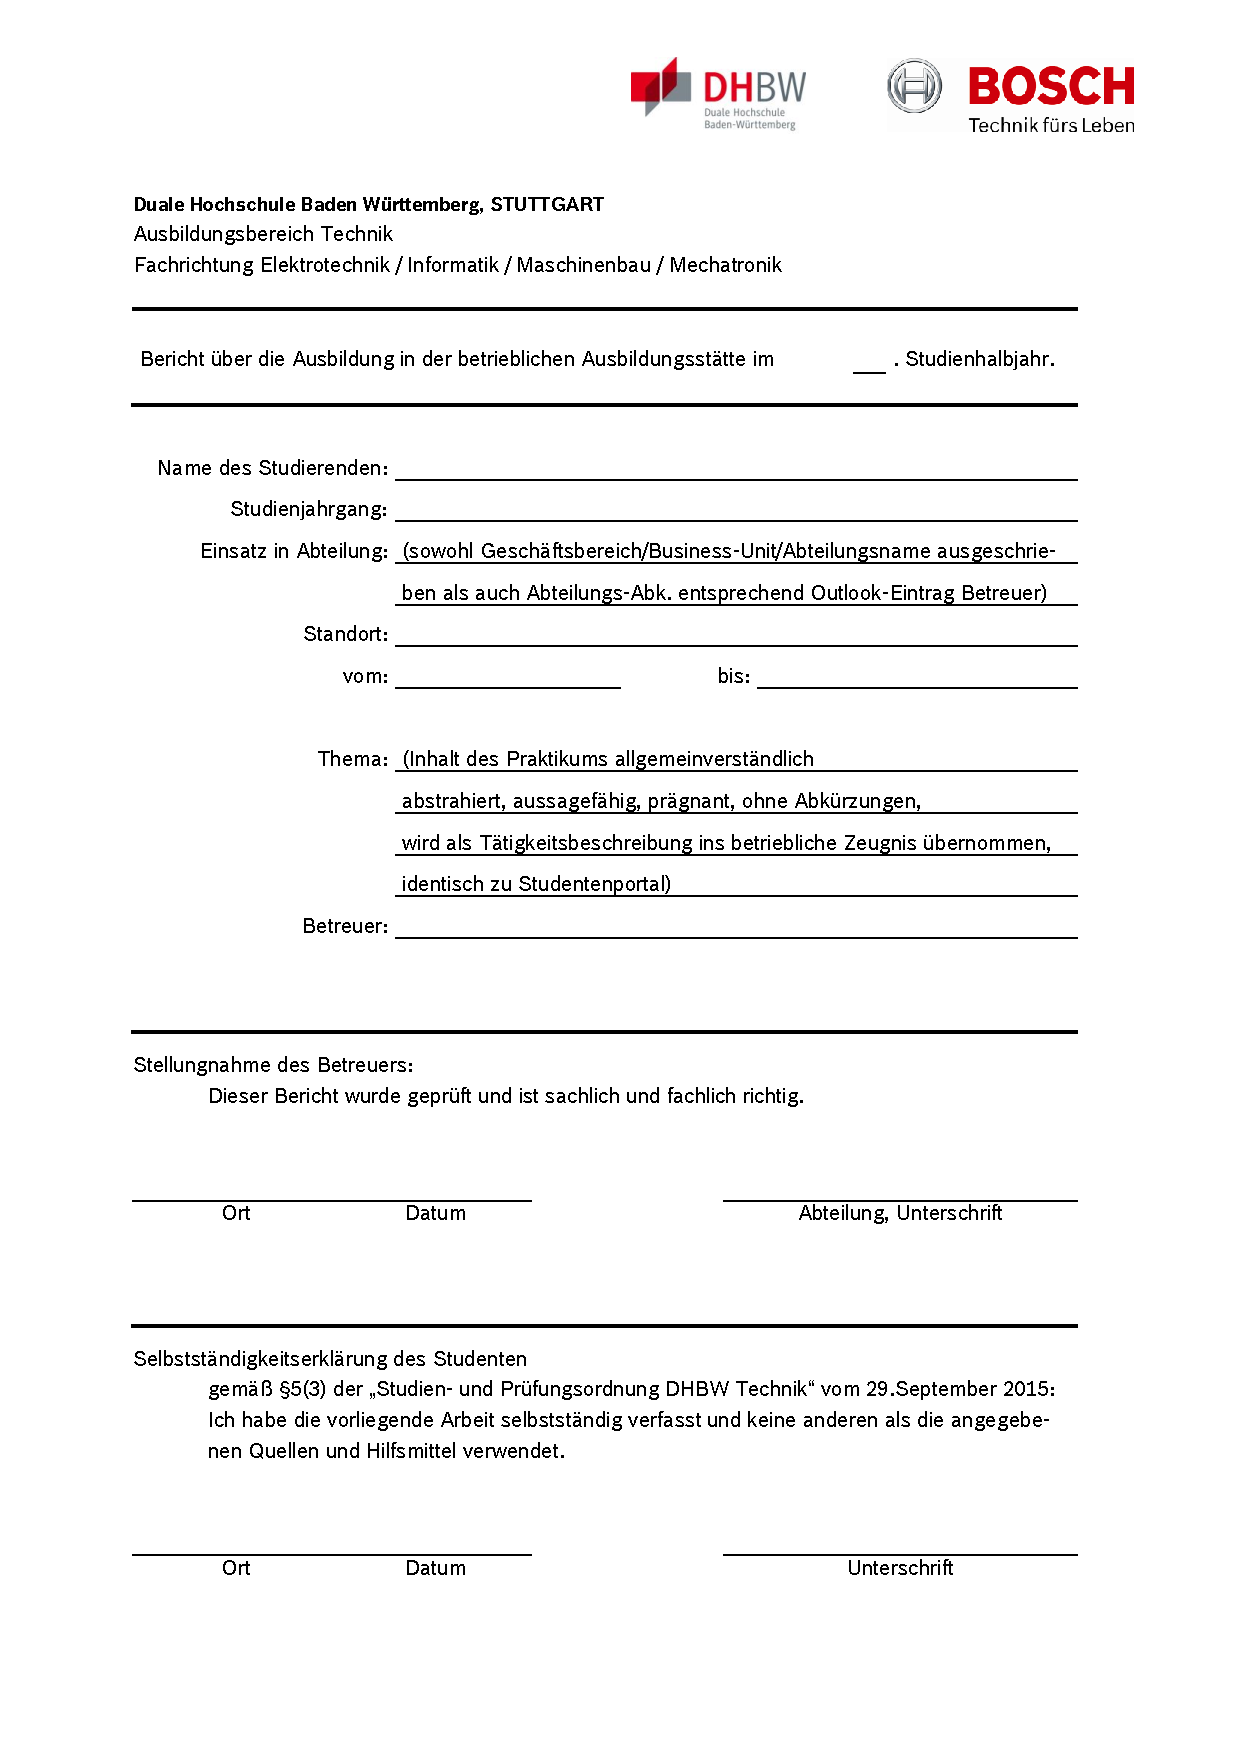
\includepdf[scale=1,clip,trim=0cm 1.5cm 0cm 2.5cm,pages={1},pagecommand={}]{ads/unterschriftenblatt}
        \newpage
    \fi

    % Selbstständigkeitserklärung nur einfügen, wenn Flag in den Einstellungen gesetzt ist
    \ifselbsterkl
        %!TEX root = ../dokumentation.tex

\thispagestyle{plain}
% Sperrvermerk direkt nach Selbstständigkeitserklärung
\section*{Selbstständigkeitserklärung}
%\section*{\\\langselbsterkl}

\vspace*{2em}


Ich versichere hiermit, dass ich meine {\arbeit} mit dem Thema: {\itshape{} \titel{}\/} selbstständig verfasst und keine anderen als die angegebenen Quellen und Hilfsmittel benutzt habe. Ich versichere zudem, dass die eingereichte elektronische Fassung mit der gedruckten Fassung übereinstimmt.

\vspace{3em}

\abgabeort, \datumAbgabe
\vspace{4em}

\begin{tabular*}{16cm}{@{\extracolsep{\fill}}>{\centering}p{6cm}c>{\centering}p{6cm}}
	\cline{1-1} \cline{3-3} 
	{Clemens Mollik} & ~ & {Jörn Herbstritt}\tabularnewline
\end{tabular*}{\footnotesize{} }{\footnotesize \par}

        \newpage
    \fi

    % Sperrvermerk
    \ifsperrvermerk
        %!TEX root = ../dokumentation.tex

\thispagestyle{plain}
% Sperrvermerk direkt hinter Titelseite
\section*{\\\langsperrvermerk}

\vspace*{2em}

\iflang{de}{%
  Die vorliegende {\arbeit} mit dem Titel \begin{center}{\itshape{}\titel{}\/}\end{center}  enthält unternehmensinterne bzw. vertrauliche Informationen der {\firma}, ist deshalb mit einem Sperrvermerk versehen und wird ausschließlich zu Prüfungszwecken am Studiengang {\studiengang} der Dualen Hochschule Baden-Württemberg {\dhbw} vorgelegt. 
	\\
	\\
	Der Inhalt dieser Arbeit darf weder als Ganzes noch in Auszügen Personen außerhalb des Prüfungsprozesses und des Evaluationsverfahrens zugänglich gemacht werden, sofern keine anders lautende Genehmigung der Ausbildungsstätte ({\firma}) vorliegt.
}

%http://www.ib.dhbw-mannheim.de/fileadmin/ms/bwl-ib/Downloads_alt/Leitfaden_31.05.pdf

\iflang{en}{%
  The {\arbeit} on hand 
  \begin{center}{\itshape{} \titel{}\/}\end{center} 
   contains internal respective confidential data of {\firma}. It is intended solely for inspection by the assigned examiner, the head of the {\studiengang} department and, if necessary, the Audit Committee \langanderdh{} {\dhbw}. It is strictly forbidden:
    \begin{itemize}
    \item to distribute the content of this paper (including data, figures, tables, charts etc.) as a whole or in extracts,
    \item to make copies or transcripts of this paper or of parts of it,
    \item to display this paper or make it available in digital, electronic or virtual form.
    \end{itemize}
  Exceptional cases may be considered through permission granted in written form by the author and {\firma}.
}

\vspace{3em}

\abgabeort, \datumAbgabe
\vspace{4em}

\rule{6cm}{0.4pt}\\
\autor

        \newpage
    \fi

    % Abstract
    \ifabstract
        %!TEX root = ../dokumentation.tex


\newcommand{\deAbstractContent}{
    Durch immer stärker werdende Computer Hardware und sinkende Preise bei Virtual Reality (VR) Systemen wird VR immer beliebter. Bisherige Eingabemethoden beschränken sich hauptsächlich auf die mitgelieferten Controller. Jedoch gibt es mittlerweile einige Firmen, die Einbaulösungen für Eye-Tracking in VR-Brillen anbieten, einige VR Brillen kommen bereits mit Eye-Tracking installiert. Die Anwendungsgebiete sind sehr zahlreich. In dieser Arbeit wird untersucht, ob Eye-Tracking als Eingabemethode geeignet ist. Dafür wurde eine Versuchsumgebung erstellt, in der zwei Zielmethoden, der klassische Laserpointer mit dem VR-Controller und Eye-Tracking, mit zwei Bestätigungsmethoden, dem Trigger des Controllers und Blinzeln, verbunden wurde. Dadurch entstehen vier Steuermethoden, die in Probandenversuchen mit vier Testpersonen getestet wurden. Der Proband muss Knöpfe in einer bestimmten Reihenfolge betätigen. Jede Steuermethode wird jeweils einmal mit großen und kleinen Knöpfen durchgeführt. Dabei werden neben dem subjektiven Empfinden auch die Genauigkeit und die Zeiten der Versuche untersucht. Dabei stellte sich die herkömmliche Kombination aus Laserpointer und Trigger als die effizienteste (schnellste und genauste) Methode heraus. Blinzeln als Bestätigungsmethode in Kombination mit dem Laserpointer konnte ähnliche Werte in diesen Kategorien erreichen. Eye-Tracking mit Trigger landete auf dem dritten Platz, konnte aber mit guten Werten, vor allem bei großen Knöpfen, überzeugen. Eye-Tracking mit Blinzeln hat mit Abstand am schlechtesten abgeschlossen und ist, in der implementierten Form, keine valide Möglichkeit zur Steuerung in VR. Ein weiterer Versuchsaufbau, basierend auf den hier erlangten Erkenntnissen, können die Eignung von Eye-Tracking zur Steuerung in größeren Probandenversuchen und angepasstem Versuchsaufbau besser darstellen. Die hier beschriebenen Ergebnisse deuten darauf hin, dass Eye-Tracking eine valide Option ist.
    \todo[inline]{CM: Alle Verzeichnisse aktualisieren und durchgehhen ob alles passt}
}

\newcommand{\enAbstractContent}{
    Increasing power in computer hardware and more competitive pricing in virtual reality (VR) lead to more and more popularity for VR systems. The input most widely used are the physical controllers coming with the VR system. However, there are more and more providers of Eye-Tracking, some providing add-on solutions, some providing built-in solutions for eye tracking in VR headsets. Eye tracking can be used in a variety of ways in VR. In this paper, the possibility of using eye-tracking as an input method is investigated. A VR environment is created, in which varying input methods are compared. For aiming the standard VR approach of a laser pointer using the physical controllers and eye tracking are compared. For input selection blinking and the trigger of the controller are used. This results in four different input methods. The input methods are compared in a trial with four participants. The study participant needs to select a pre-defined sequence of buttons with each input method. Each input method is tested once with small and once with big buttons. To compare the different input methods, the subjects are asked about their experience and data like the accuracy and the times to complete the tasks are measured and analyzed. The combination laser pointer/trigger with the physical controller proofed to be the most effective way of navigating the test level. Using blinking instead of the trigger in combination with the laser pointer proofed to be almost as effective. Eye tracking used with the trigger of the controller showed to be a viable way of navigating the level but fell short of the two variants using the laser pointer. The combination of eye tracking and blinking proofed far worse than all other input methods and should, in the current implementation, not be used for controlling environments in VR. This paper is meant as a reference point for future studies using eye tracking as input method. The results are promising, although further research is required. 
}

%%%%%%%% Ab hier nicht mehr anfassen! %%%%%%%%

\newcommand{\deAbstract}{%
    \renewcommand{\abstractname}{\langabstract} % Text für Überschrift
    \begin{abstract}
        \thispagestyle{plain}
        \deAbstractContent
    \end{abstract}
}

\newcommand{\enAbstract}{
    \renewcommand{\abstractname}{\langabstract} % Text für Überschrift
    \begin{abstract}
        \thispagestyle{plain}
        \enAbstractContent
    \end{abstract}
}

\iflang{de}{
    \deAbstract
    \ifbothabstracts
        \clearpage
      %  \begin{otherlanguage}{english}
            \enAbstract
     %   \end{otherlanguage}
    \fi
}

\iflang{en}{
    \enAbstract
    \ifbothabstracts
        \clearpage
        \begin{otherlanguage}{ngerman}
            \deAbstract
        \end{otherlanguage}
    \fi
}
        \newpage
    \fi

    \pagestyle{plain}		% nur Seitenzahlen im Fuß

    %\RedeclareSectionCommand[beforeskip=\kapitelabstand]{chapter} 
    % Inhaltsverzeichnis
    \ifinhalt
        \begin{spacing}{1.1}
            \begingroup
                % auskommentieren für Seitenzahlen unter Inhaltsverzeichnis
                % \renewcommand*{\chapterpagestyle}{empty}
                % \pagestyle{plain}
                    
                    
                %\setcounter{tocdepth}{1}
                %für die Anzeige von Unterkapiteln im Inhaltsverzeichnis
                %\setcounter{tocdepth}{2}
                \pdfbookmark{\contentsname}{toc}
                \tableofcontents
                \clearpage
            \endgroup
        \end{spacing}
        \newpage
    \fi

    % Abkürzungsverzeichnis
    \ifabkverz
        \cleardoublepage
        \addchap{\langabkverz}

        \begin{acronym}[LOREMIPSUM] % Die Angabe in eckigen Klammern legt die Breite der linken Spalte fest! => ggf. anpassen
            \IfFileExists{{ads/sortedAcronyms}}{%		\acf{Abk.}   --> fügt die Abkürzung UND die Erklärung ein
%		\acl{Abk.}   --> fügt nur die Erklärung ein
%		\acp{Abk.}  --> gibt Plural aus (angefügtes 's'); das zusätzliche 'p' funktioniert auch bei obigen Befehlen
%		\acs{Abk.}   -->  fügt die Abkürzung ein
%		\ac{Abk.}   --> fügt die Abkürzung ein, beim ersten Aufruf wird zusätzlich automatisch die ausgeschriebene Version davor eingefügt bzw. in einer Fußnote (hierfür muss in header.tex \usepackage[printonlyused,footnote]{acronym} stehen) dargestellt
%	siehe auch: http://golatex.de/wiki/%5Cacronym
%!TEX root = ../dokumentation.tex
%Verwendung: 
%nur verwendete Akronyme werden letztlich im Abkürzungsverzeichnis des Dokuments angezeigt
\acro{AMOLED}{Active Matrix Organic Light Emitting Diode}
\acro{AR}{Augmented Reality}
\acro{BSP}{Board Support Package} % Beispielabkürzung
\acro{COVID-19}{Coronavirus Disease 2019}
\acro{HMD}{Head-Mounted Display}
\acro{MR}{Mixed Reality}
\acro{MT}{Movement Time}
\acro{SDK}{Software Development Kit}
\acro{VR}{Virtual Reality}
\acro{u}{Unity Einheit}
}{%!TEX root = ../dokumentation.tex
%nur verwendete Akronyme werden letztlich im Abkürzungsverzeichnis des Dokuments angezeigt
%Verwendung: 
%		\ac{Abk.}   --> fügt die Abkürzung ein, beim ersten Aufruf wird zusätzlich automatisch die ausgeschriebene Version davor eingefügt bzw. in einer Fußnote (hierfür muss in header.tex \usepackage[printonlyused,footnote]{acronym} stehen) dargestellt
%		\acs{Abk.}   -->  fügt die Abkürzung ein
%		\acf{Abk.}   --> fügt die Abkürzung UND die Erklärung ein
%		\acl{Abk.}   --> fügt nur die Erklärung ein
%		\acp{Abk.}  --> gibt Plural aus (angefügtes 's'); das zusätzliche 'p' funktioniert auch bei obigen Befehlen
%	siehe auch: http://golatex.de/wiki/%5Cacronym
\acro{BSP}{Board Support Package} % Beispielabkürzung
\acro{VR}{Virtual Reality}
\acro{AR}{Augmented Reality}
\acro{MR}{Mixed Reality}
\acro{HMD}{Head-Mounted Display}
\acro{CBA}{CBA}
\acro{MT}{Movement Time}}
        \end{acronym}
    \fi

    % Abbildungsverzeichnis
    \ifabbverz
        \cleardoublepage
        \listoffigures
    \fi

    % Tabellenverzeichnis
    \iftableverz
        \cleardoublepage
        \listoftables
    \fi

	% Formelgrößenverzeichnis
	\ifformelgroeverz
		\cleardoublepage
		\addchap{\langformelgroeverz}
		
		\begin{acronym}[LOREMIPSUM] % Die Angabe in eckigen Klammern legt die Breite der linken Spalte fest! => ggf. anpassen
			%!TEX root = ../dokumentation.tex

% Verwendung im Text analog zu Akronymen --> siehe ads/acronyms.tex für mehr Info)

\newcommand{\acrounit}[1]{
	\acroextra{\makebox[35mm][l]{#1}}
}

\acro{a}[$a$]{\acrounit{rad}Bedeutung von a}
\acro{b}[$b$]{\acrounit{rad}Bedeutung von b}
\acro{lambda}[$\lambda$]{\acrounit{rad}Bedeutung von lambda}
\acro{phi}[$\phi$]{\acrounit{rad}Bedeutung von phi}
		\end{acronym}
	\fi

    % Formelverzeichnis
    % mit "\formelentry{Formelname}" können neue Einträge erstellt werden. => auslagern in separates File? z.B. \input{ads/formels}
    \ifformelverz
        \cleardoublepage
        \listofformels
    \fi

    % Listingsverzeichnis
    \iflistverz
        \cleardoublepage
        \lstlistoflistings
    \fi

    \label{endOfRomanNumbering}

    \cleardoublepage

    %begin of new numbering
    \setpagestylecontent

    % Inhalt
    \foreach \i in {01,02,03,04,05,06,07,08,09,...,99} {%
        \edef\FileName{content/\i kapitel}%
            \IfFileExists{\FileName}{%
                \input{\FileName}
                
            }
            {%
                %file does not exist
            }
    }
    \label{endOfArabicNumbering}
    \clearpage

    \ifappendix
        %!TEX root = ../dokumentation.tex

\section{Klassendiagramm}

\begin{figure}[!htbp]
	\centering
	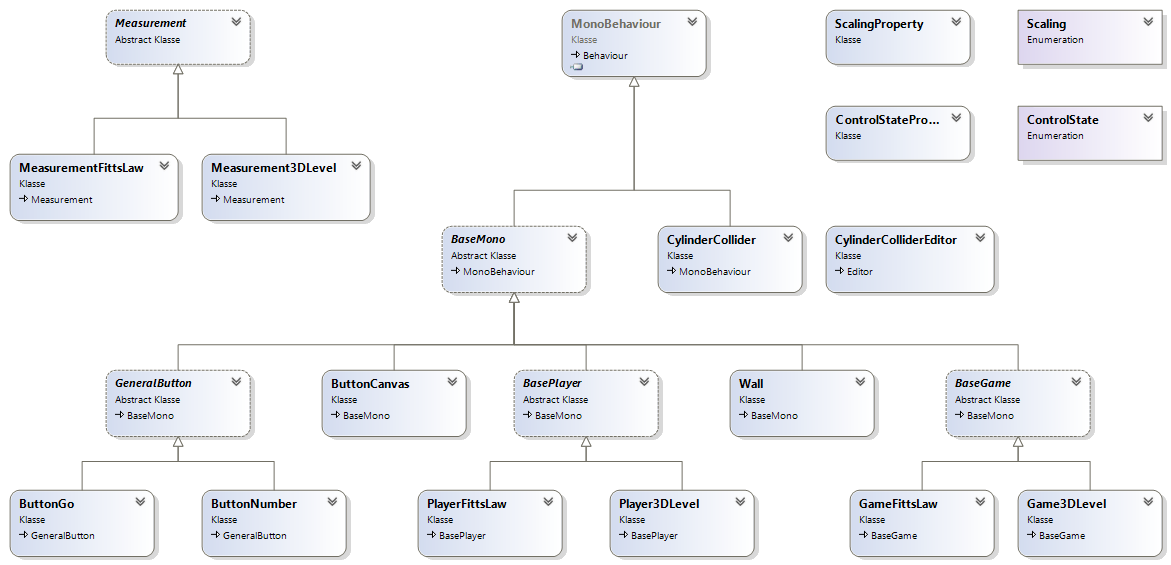
\includegraphics[angle=90,height=0.9\textheight]{ClassDiagram}
	\caption[Übersicht Klassenhierarchie]{Übersicht Klassenhierarchie}
	\label{fig:ClassDiagram}
\end{figure}

\section{Tabelle der Versuche}
% Please add the following required packages to your document preamble:
% \usepackage{booktabs}
% \usepackage{graphicx}

\begin{table}[H]	
	\caption{Tabelle der Versuche}
	\label{table:probanden}
	\resizebox{\textwidth}{!}{%
		\begin{tabular}{@{}lllll@{}}
			\toprule
			Proband & Laserpointer und Trigger & Laserpointer und Blinzeln & Eye-Tracking und Trigger & Eye-Tracking und Blinzeln \\ \midrule
			1  & (3, 2), (2, 2), (3, 3) & (3, 2), (1, 2), (3, 3) & (3, 4), (2, 4), (3, 2) & (2, 3), (1, 3), (2, 1) \\
			2  & (1, 3), (3, 3), (1, 4) & (2, 1), (1, 1), (2, 3) & (1, 3), (2, 3), (1, 2) & (3, 2), (1, 2), (3, 4) \\
			3  & (1, 4), (2, 4), (1, 3) & (1, 4), (3, 4), (1, 3) & (1, 1), (2, 1), (1, 3) & (1, 4), (2, 4), (1, 3) \\
			4  & (3, 4), (1, 4), (3, 1) & (2, 4), (3, 4), (2, 1) & (2, 3), (3, 3), (2, 2) & (1, 1), (3, 1), (1, 2) \\
			5  & (3, 1), (1, 1), (3, 3) & (2, 3), (3, 3), (2, 4) & (1, 3), (3, 3), (1, 2) & (3, 1), (1, 1), (3, 2) \\
			6  & (2, 2), (3, 2), (2, 3) & (3, 1), (2, 1), (3, 4) & (3, 2), (1, 2), (3, 1) & (2, 2), (3, 2), (2, 3) \\
			7  & (2, 1), (3, 1), (2, 4) & (2, 2), (3, 2), (2, 4) & (2, 4), (3, 4), (2, 2) & (3, 3), (2, 3), (3, 2) \\
			8  & (2, 4), (3, 4), (2, 3) & (2, 1), (3, 1), (2, 4) & (2, 3), (3, 3), (2, 4) & (3, 4), (1, 4), (3, 3) \\
			9  & (1, 1), (2, 1), (1, 4) & (1, 2), (2, 2), (1, 4) & (2, 1), (1, 1), (2, 2) & (1, 2), (2, 2), (1, 1) \\
			10 & (3, 1), (2, 1), (3, 3) & (1, 2), (3, 2), (1, 3) & (3, 1), (2, 1), (3, 3) & (2, 1), (1, 1), (2, 2) \\
			11 & (2, 1), (3, 1), (2, 4) & (3, 1), (1, 1), (3, 3) & (1, 4), (2, 4), (1, 2) & (2, 2), (3, 2), (2, 4) \\
			12 & (1, 4), (3, 4), (1, 1) & (1, 1), (3, 1), (1, 4) & (3, 4), (1, 4), (3, 1) & (2, 4), (3, 4), (2, 3) \\
			13 & (1, 2), (2, 2), (1, 1) & (2, 2), (1, 2), (2, 3) & (3, 1), (1, 1), (3, 2) & (1, 4), (3, 4), (1, 2) \\
			14 & (3, 2), (2, 2), (3, 4) & (2, 2), (3, 2), (2, 3) & (3, 4), (1, 4), (3, 2) & (3, 3), (1, 3), (3, 1) \\
			15 & (3, 3), (2, 3), (3, 2) & (1, 4), (3, 4), (1, 3) & (2, 1), (1, 1), (2, 2) & (2, 1), (3, 1), (2, 4) \\
			16 & (1, 3), (2, 3), (1, 2) & (1, 3), (3, 3), (1, 4) & (3, 4), (1, 4), (3, 1) & (2, 1), (3, 1), (2, 2) \\
			17 & (1, 2), (2, 2), (1, 1) & (2, 1), (1, 1), (2, 4) & (2, 2), (1, 2), (2, 3) & (1, 4), (2, 4), (1, 1) \\
			18 & (2, 4), (3, 4), (2, 1) & (3, 3), (1, 3), (3, 4) & (1, 3), (2, 3), (1, 1) & (1, 4), (3, 4), (1, 3) \\
			19 & (1, 2), (3, 2), (1, 3) & (2, 2), (1, 2), (2, 3) & (2, 4), (1, 4), (2, 1) & (1, 3), (3, 3), (1, 2) \\
			20 & (1, 3), (2, 3), (1, 2) & (3, 1), (1, 1), (3, 2) & (3, 3), (1, 3), (3, 2) & (2, 3), (3, 3), (2, 1) \\ \bottomrule
		\end{tabular}%
	}
\end{table}

\section{Tabellen der Befragungsergebnisse}

\begin{table}[]
	\resizebox{\textwidth}{!}{%
		\begin{tabular}{|l|l|l|l|l|}
			\hline
			\multirow{2}{*}{Proband} & \multicolumn{4}{l|}{Eye-Tracking/Trigger}                         \\ \cline{2-5} 
			& Fixierung & Auswahl & Eignung Menüsteuerung & Einfluss Knopfgröße \\ \hline
			Proband 1                & 5         & 5       & 5                     & 2                   \\ \hline
			Proband 2                & 5         & 5       & 5                     & 2                   \\ \hline
			Proband 3                & 5         & 5       & 5                     & 2                   \\ \hline
			Proband 4                & 5         & 5       & 5                     & 2                   \\ \hline
		\end{tabular}%
	}
\end{table}

\begin{table}[]
	\resizebox{\textwidth}{!}{%
		\begin{tabular}{|l|l|l|l|l|}
			\hline
			\multirow{2}{*}{Proband} & \multicolumn{4}{l|}{Laserpointer/Blinzeln}                        \\ \cline{2-5} 
			& Fixierung & Auswahl & Eignung Menüsteuerung & Einfluss Knopfgröße \\ \hline
			Proband 1                & 5         & 3       & 4                     & 3                   \\ \hline
			Proband 2                & 5         & 4       & 5                     & 2                   \\ \hline
			Proband 3                & 5         & 5       & 4                     & 2                   \\ \hline
			Proband 4                & 5         & 1       & 1                     & 2                   \\ \hline
		\end{tabular}%
	}
\end{table}

\begin{table}[]
	\resizebox{\textwidth}{!}{%
		\begin{tabular}{|l|l|l|l|l|}
			\hline
			\multirow{2}{*}{Proband} & \multicolumn{4}{l|}{Eye-Tracking/Trigger}                         \\ \cline{2-5} 
			& Fixierung & Auswahl & Eignung Menüsteuerung & Einfluss Knopfgröße \\ \hline
			Proband 1                & 3         & 4       & 4                     & 4                   \\ \hline
			Proband 2                & 4         & 4       & 5                     & 3                   \\ \hline
			Proband 3                & 2         & 4       & 3                     & 4                   \\ \hline
			Proband 4                & 4         & 4       & 5                     & 4                   \\ \hline
		\end{tabular}%
	}
\end{table}

\begin{table}[]
	\resizebox{\textwidth}{!}{%
		\begin{tabular}{|l|l|l|l|l|}
			\hline
			\multirow{2}{*}{Proband} & \multicolumn{4}{l|}{Eye-Tracking/Blinzeln}                         \\ \cline{2-5} 
			& Fixierung & Auswahl & Eignung Menüsteuerung & Einfluss Knopfgröße \\ \hline
			Proband 1                & 1         & 1       & 1                     & 5                   \\ \hline
			Proband 2                & 1         & 1       & 1                     & 5                   \\ \hline
			Proband 3                & 2         & 1       & 1                     & 5                   \\ \hline
			Proband 4                & 1         & 1       & 1                     & 5                   \\ \hline
		\end{tabular}%
	}
\end{table}

\begin{table}[]
	\resizebox{\textwidth}{!}{%
		\begin{tabular}{|l|l|l|l|l|}
			\hline
			\multirow{2}{*}{Proband} &
			\multicolumn{4}{l|}{Ranking und Begründung} \\ \cline{2-5} 
			&
			Ranking &
			Begründung 1. Platz &
			Begründung 2. Platz &
			Begründung 4. Platz \\ \hline
			Proband 1 &
			1, 2, 3, 4 &
			\begin{tabular}[c]{@{}l@{}}Fühlt sich intuitiv an, ist \\ am einfachsten zu bedienen \\ und funktioniert auf Anhieb.\end{tabular} &
			\begin{tabular}[c]{@{}l@{}}das Blinzeln als Alternative \\ zum Trigger hat \\ auch sehr gut funktioniert.\end{tabular} &
			\begin{tabular}[c]{@{}l@{}}Eye-Tracking mit Blinzeln \\ hat überhaupt nicht funktioniert \\ und war eines der qualvollsten \\ Erlebnisse meines Lebens.\end{tabular} \\ \hline
			Proband 2 &
			1, 2, 3, 4 &
			\begin{tabular}[c]{@{}l@{}}Für mich als geübten \\ VR-Nutzer mit Abstand \\ am intuitivsten\end{tabular} &
			\begin{tabular}[c]{@{}l@{}}Die Genauigkeit der \\ Laserpointers mit der einfachen \\ Interaktion durch blinzeln hat \\ sehr gut funktioniert\end{tabular} &
			\begin{tabular}[c]{@{}l@{}}Fixierung war sehr schwer, \\ ich habe oft nicht den Knopf \\ getroffen, den ich treffen wollte. \\ Beim Blinzeln ist die Position \\ des Eye-Trackers oft verrutscht, \\ so dass ein genaues Treffen der \\ Knöpfe praktisch unmöglich war\end{tabular} \\ \hline
			Proband 3 &
			1, 2, 3, 4 &
			\begin{tabular}[c]{@{}l@{}}Beim Laserpointer wusste \\ man immer genau wohin \\ man zielte. Das Bestätigen \\ mit dem Trigger funktionierte \\ immer direkt auf Anhieb.\end{tabular} &
			\begin{tabular}[c]{@{}l@{}}Der Unterschied zu Nummer 1 \\ ist, dass das Blinzeln nicht \\ immer direkt auf Anhieb \\ funktionierte oder bei einem \\ unbewussten Blinzeln aktiviert \\ wurde.\end{tabular} &
			\begin{tabular}[c]{@{}l@{}}Die Kombination aus Eye-Tracking \\ und Blinzeln ist eine ziemlich \\ schwierige Angelegenheit. Das \\ Anvisieren eines Punktes mit \\ Eye-Tracking ist ziemlich \\ anstrengend und dauert deutlich \\ länger als mit dem Laserpointer. \\ Wenn man es endlich geschafft hatte \\ den gewünschten Button auszuwählen \\ und mittels Blinzeln bestätigen wollte, \\ verrutschte der anvisierte Punkte und \\ etwas anderes wurde ausgewählt.\end{tabular} \\ \hline
			Proband 4 &
			1, 3, 2, 4 &
			Hat am besten funktioniert &
			\begin{tabular}[c]{@{}l@{}}Hat meist gut funktioniert, \\ aber nicht so verlässlich wie \\ Laserpointer/Trigger\end{tabular} &
			\begin{tabular}[c]{@{}l@{}}Eye-Tracking hat oft nicht gut \\ funktioniert, Blinzeln zum bestätigen \\ hat sehr viele Versuche gebraucht\end{tabular} \\ \hline
		\end{tabular}%
	}
\end{table}


\section{Gesamtdauer mit kleinen Knöpfen}
\label{appendix:timessmall}
\begin{figure}[!htbp]
	\centering
	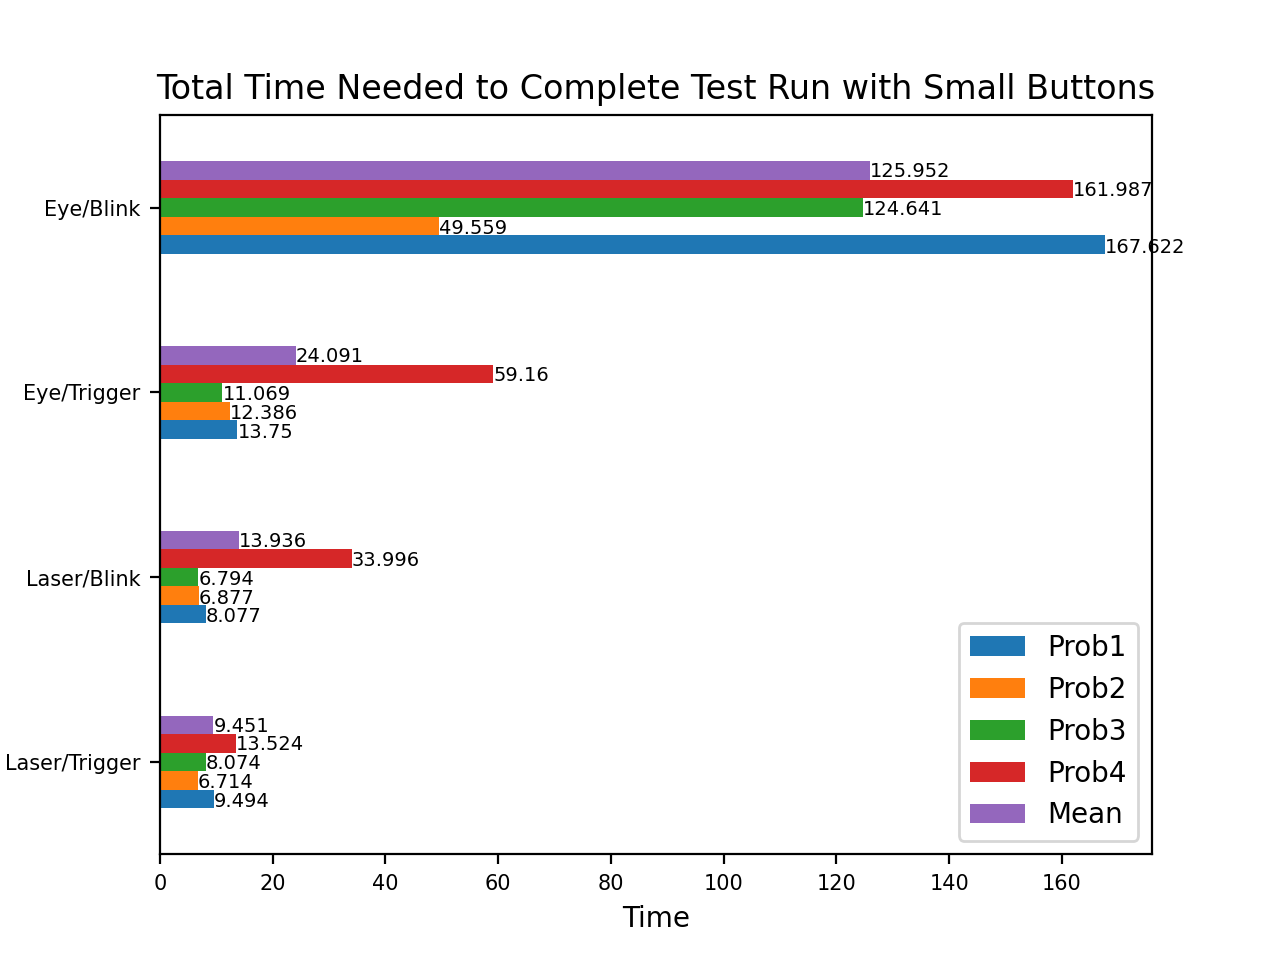
\includegraphics[width=1.0\linewidth]{plot_small}
	\caption[Gesamtdauer eines Versuchdurchlaufs pro Steuerart pro Proband und im Durchschnitt bei kleinen Knöpfen] {Gesamtdauer eines Versuchdurchlaufs pro Steuerart pro Proband und im Durchschnitt bei kleinen Knöpfen}
\end{figure}

\section{Eye-Tracking Heatmaps der Probandenversuche}
\label{appendix:heatmaps}
\begin{figure}[!htbp]
	\centering
	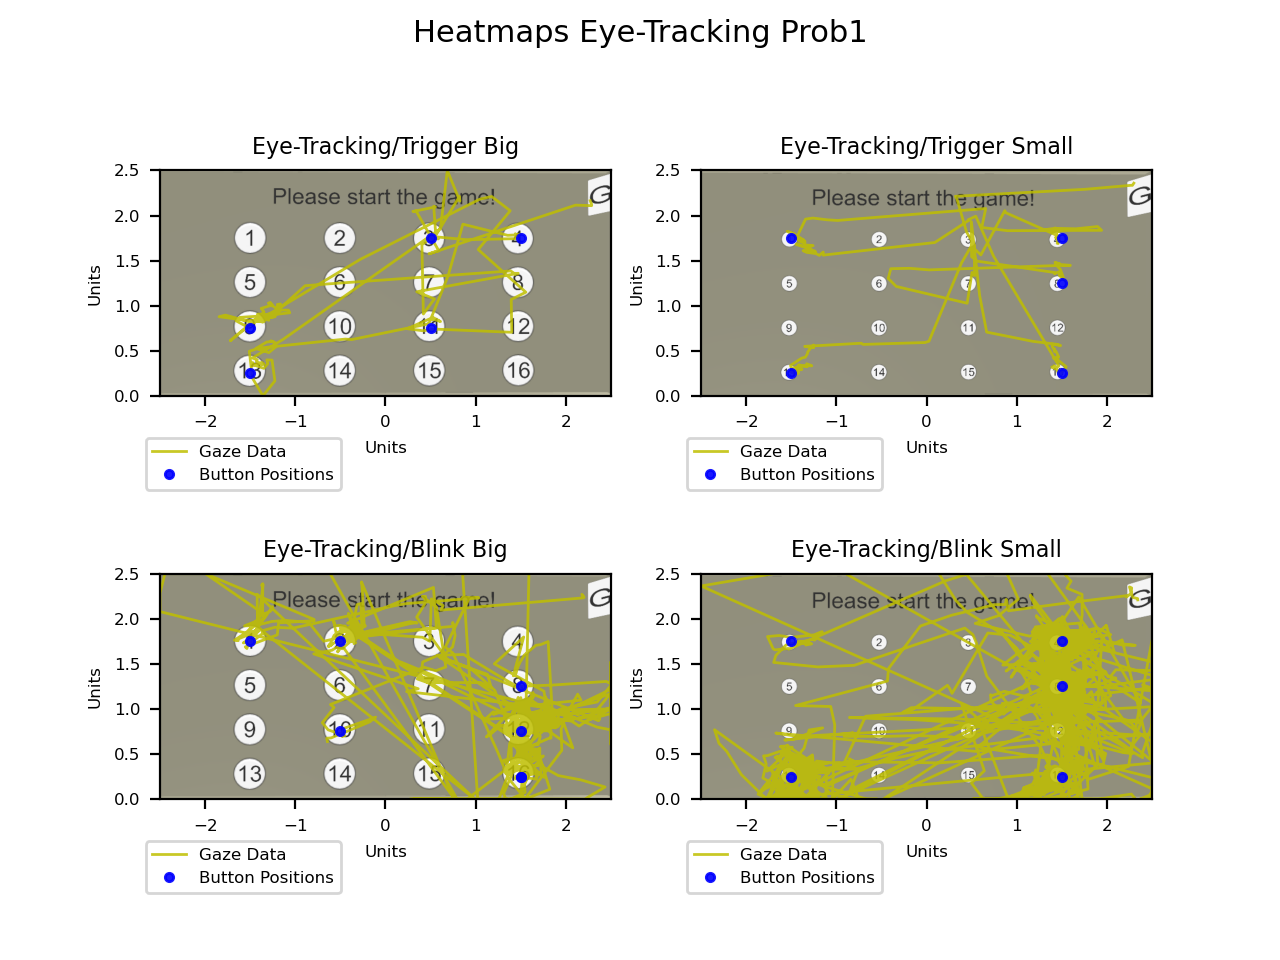
\includegraphics[width=1.0\linewidth]{plot_heatmap_prob1}
	\caption[Visualisierung der Blickdaten und der auszuwählenden Knöpfe] {Visualisierung der Blickdaten und der auszuwählenden Knöpfe}
\end{figure}
\begin{figure}[!htbp]
	\centering
	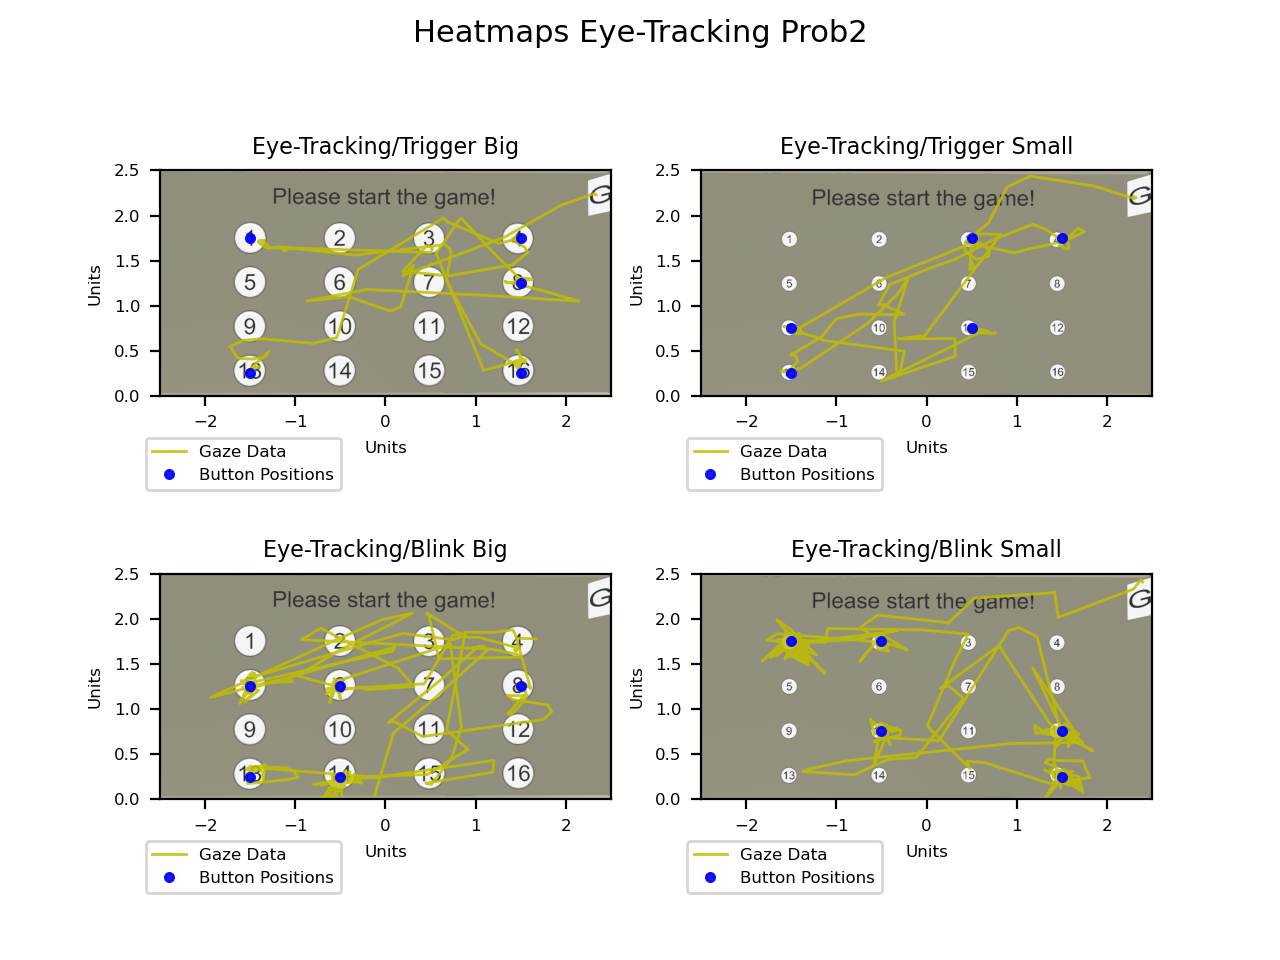
\includegraphics[width=1.0\linewidth]{plot_heatmap_prob2}
	\caption[Visualisierung der Blickdaten und der auszuwählenden Knöpfe] {Visualisierung der Blickdaten und der auszuwählenden Knöpfe}
\end{figure}
\begin{figure}[!htbp]
	\centering
	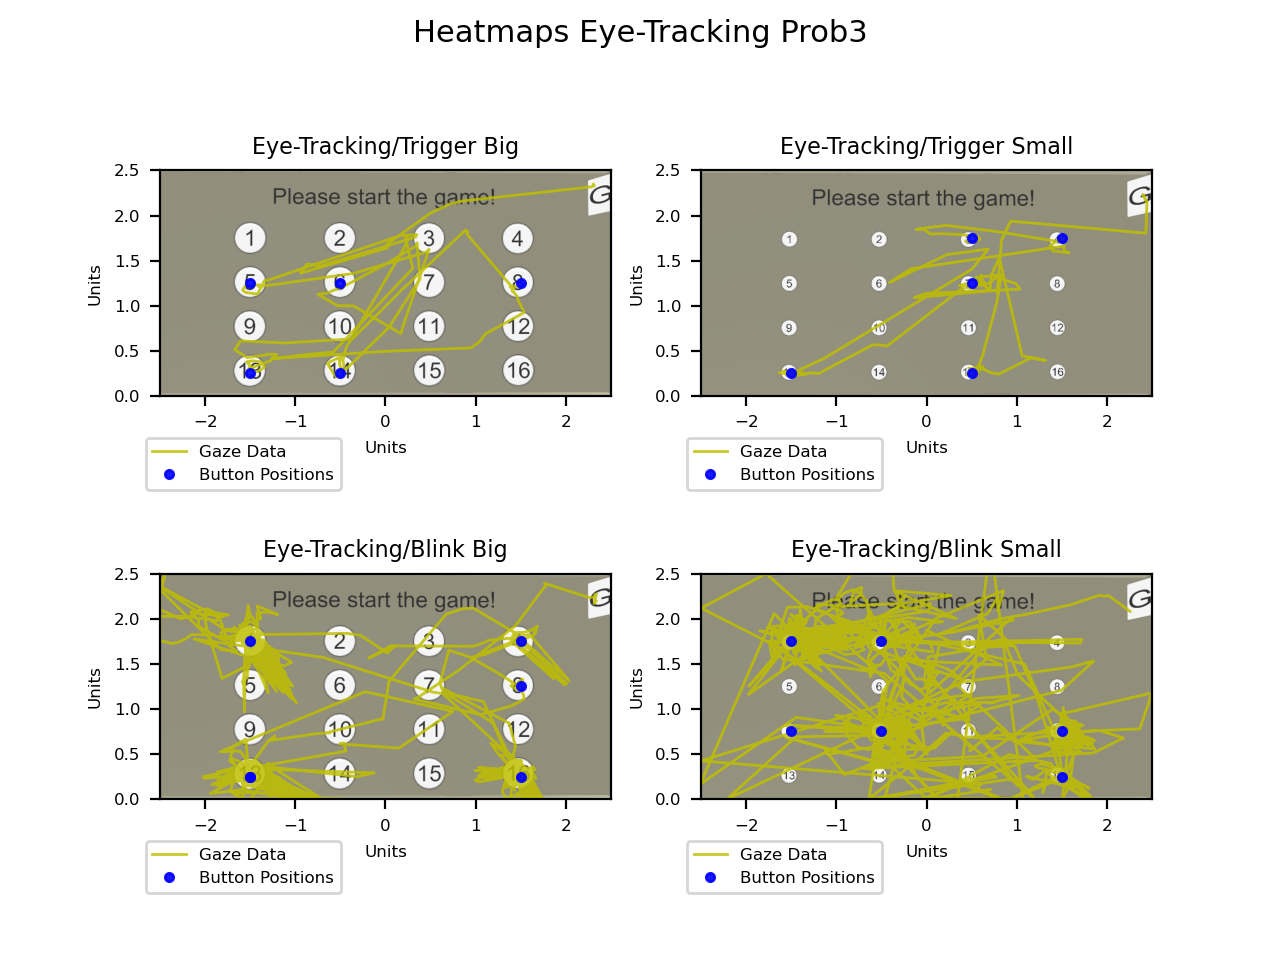
\includegraphics[width=1.0\linewidth]{plot_heatmap_prob3}
	\caption[Visualisierung der Blickdaten und der auszuwählenden Knöpfe] {Visualisierung der Blickdaten und der auszuwählenden Knöpfe}
\end{figure}
\begin{figure}[!htbp]
	\centering
	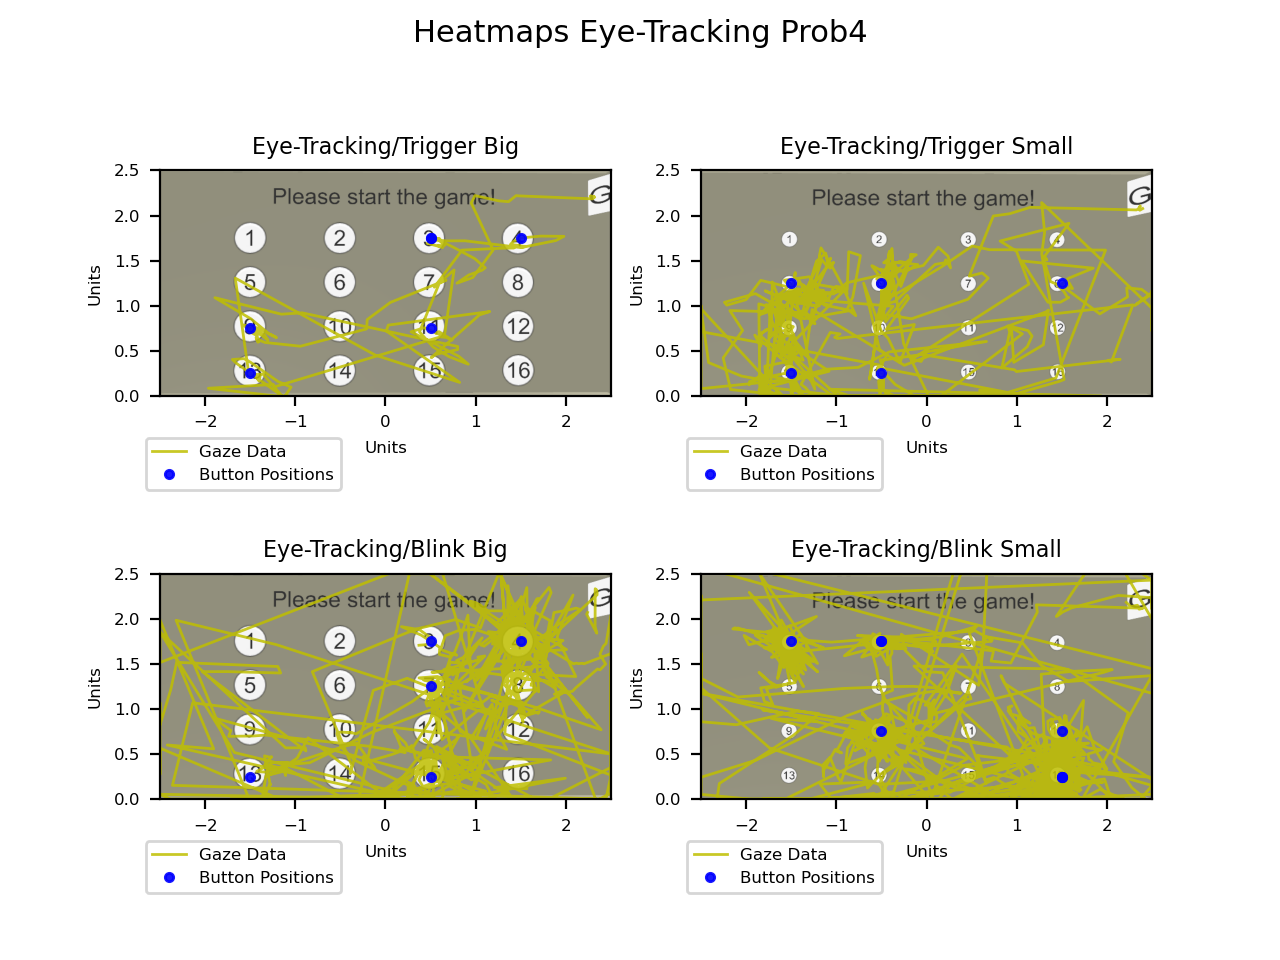
\includegraphics[width=1.0\linewidth]{plot_heatmap_prob4}
	\caption[Visualisierung der Blickdaten und der auszuwählenden Knöpfe] {Visualisierung der Blickdaten und der auszuwählenden Knöpfe}
\end{figure}
    \fi
\end{document}
